\chapter{Framework LuaOnTV 2.0} \label{cap:luaontv}
Atendendo ao requisito "T3) Facilitar o desenvolvimento de aplicações interativas"  apresentado na Seção \ref{sec:req-arquitetura},
foi utilizado o \textit{framework} LuaOnTV, como ponto de partida, no qual foram realizadas melhorias a serem apresentadas neste capítulo.

O LuaOnTV\cite{junior2009luacomp} é um \textit{framework} para facilitar o desenvolvimento de aplicações procedurais
para o Sistema Brasileiro de TV Digital, utilizando a linguagem Lua, por meio
de \textit{scripts} NCLua (\textit{scripts} Lua embutidos em documentos NCL).
O mesmo foi resultado de trabalho de projeto de pesquisa desenvolvido por equipe do Laboratório de TV Digital Interativa da
Universidade de Brasília, sob orientação do professor Paulo Roberto de Lira Gondim. 
Ele foi um projeto pioneiro para o SBTVD, desenvolvido inteiramente em linguagem Lua,
sob o paradigma de programação orientada a objetos, que disponibiliza um conjunto
de classes e componentes visuais e não visuais para o desenvolvimento
de aplicações interativas para TVD.

Os componentes do LuaOnTV utilizam os módulos \textit{canvas} e \textit{event} existentes em NCLua.
Tais módulos estendem as funcionalidades da linguagem Lua para o contexto de TV Digital.
Desta forma, o \textit{framework} está totalmente em conformidade com as normas do Ginga-NCL.
O \textit{framework} tem como principal objetivo facilitar a construção de interfaces gráficas
para aplicações interativas, disponibilizando componentes para entrada e saída de dados, 
além de automatizar o processo de controle de foco.

Os componentes visuais foram desenvolvidos com base nos componentes 
existentes em diferentes linguagens de programação e ambientes integrados de desenvolvimento (IDE's)
como \textit{NetBeans}, Eclipse, Adobe \textit{Dreamweaver}, \textit{Delphi}, \textit{Visual Studio} e outros; além de ferramentas
específicas para TV Digital como \textit{Jame Author} e \textit{Cardinal Studio}.

\cite{junior2009luacomp} compararam uma aplicação desenvolvida utilizando a NCL como linguagem principal e outra
utilizando o LuaOnTV, que tem a linguagem Lua como principal, e constataram que:

\begin{quote}
"uma aplicação com códigos NCL e imagens que simulam os componentes gráficos do LuaOnTV chegou a quase 1,5MB. A
mesma aplicação desenvolvida com LuaOnTV chegou a pouco mais de 60 KB."
\end{quote}

Eles também comentam que o \textit{framework} tem como um dos requisitos não funcionais 
a diminuição do tamanho do código das aplicações interativas, considerando
as capacidades restritas de memória e armazenamento dos conversores de TV Digital.
Tal requisito foi alcançado devido à utilização do paradigma de orientação a objetos, que
permite uma alta reutilização de código.


\section{Delimitação do Problema}

Devido à linguagem NCL ser uma linguagem apenas declarativa,
funcionando como uma linguagem de cola para diferentes tipos de mídias
(como GIF, JPEG, MPEG, PNG, XHTML, e outros, não restringindo nem prescrevendo nenhum
tipo de mídia)\cite{abnt200815606}, ela é uma linguagem de maior nível de abstração,
não decompondo o resultado em uma implementacão algorítmica\cite{barbosa2008tv}.
No entanto, tal linguagem não permite realização de tarefas específicas como
operações aritméticas, utilização direta de protocolos de comunicação como 
TCP, HTTP e SOAP, manipulação de arquivos, 
muito menos a definição de procedimentos (rotinas/funções).
Desta forma, a realização de tais tarefas só é possível por meio de uma linguagem
procedural como a linguagem Lua. 

No caso de entrada de dados, apesar do sub-sistema Ginga-NCL do \textit{middleware} Ginga especificar 
um recurso de teclado virtual a ser utilizado por aplicações NCL\cite{abnt200815606},
a implementação de referência do mesmo\cite{ginga-ncl-community} 
ainda não inclui tal recurso. 
Além disto, a manipulação de dados (armazenamento e obtenção) em documentos
NCL não é tão trivial como a inclusão de mídias como imagens e vídeos.

Em NCL é possível até mesmo definir o controle de foco entre campos
(por meio dos atributos \textit{moveLeft, moveRight, moveUp, moveDown}, da \textit{tag descriptor}\cite{abnt200815606})
permitindo que o usuário navegue de um campo a outro utilizando as setas
do controle remoto. No entanto, a definição da navegação entre os campos
é feita de forma completamente manual, e a inclusão ou remoção
de um novo campo no meio dos campos existentes requer a 
redefinição da ordem de navegação entre os mesmos, o que
pode ser um trabalho cansativo e suscetível a erros.

Os módulos de NCLua, utilizados pelo LuaOnTV, disponibilizam apenas um conjunto de funções básicas
específicas. Existem 5 módulos, como apresentados a seguir\cite{abnt200815606}:

\begin{itemize}
	\item \textbf{\textit{canvas}}: oferece uma API para desenhar primitivas gráficas e manipular imagens;
  \item \textbf{\textit{event}}: permite que aplicações NCLua comuniquem-se com o \textit{middleware} através de eventos (eventos NCL e de teclas);
  \item \textbf{\textit{settings}}: exporta uma tabela com variáveis definidas pelo autor do documento NCL e variáveis
 de ambiente reservadas em um nó \textit{"application/x-ginga-settings"};
  \item \textbf{\textit{persistent}}: exporta uma tabela com variáveis persistentes, que estão disponíveis para manipulação
    apenas por objetos procedurais.
\end{itemize}

A utilização direta das funções destes módulos requer um conhecimento mais profundo dos mesmos,
como temos provado durante a pesquisa e estudos de tais módulos, para o desenvolvimento
de aplicações. As funcionalidades de captura de teclas (providas pelo módulo \textit{event}) 
para entrada de dados alfabéticos e numéricos, da mesma forma como em um teclado de celular
(devido o controle remoto só possuir teclas numéricas) não é trivial. O controle de foco
a partir da captura do pressionamento das teclas direcionais do controle também é 
complicado e requer a inclusão de muito código. Tais dificuldades têm se provado verdade
pelos diversos relatos de usuários, como no Fórum da Comunidade Ginga no Portal do \textit{Software} Público\cite{ginga-ncl-community},
além de outros grupos de discussão acompanhados.

Com todas as dificuldades apresentadas, o LuaOnTV se mostrou ser uma solução ideal para a redução
da quantidade de código para a criação de aplicações procedurais com interface gráfica para a TVD, 
permitindo encapsular toda a complexidade envolvida na utilização direta dos módulos
de NCLua para chegar ao mesmo fim.

\section{LuaOnTV 2.0: Nova versão implementada}

Da mesma forma que todo projeto de \textit{software}, foi implementada e liberada uma primeira versão do LuaOnTV. 
Como extensão do trabalho de mestrado onde foi originado o mesmo, 
verificou-se que eram necessárias algumas melhorias e correções de alguns
bugs encontrados. Nesta seção será apresentada a versão 2.0
do LuaOnTV, que traz uma série de importantes novos recursos.

A seguir são listados os requisitos funcionais e não funcionais, inicialmente identificados e implementados.

\begin{center}
\scriptsize {
	\begin{tabular}{|p{11cm}|c|c|}%{|l|l|l|}
    \hline
		\textbf{Requisito} & \textbf{Funcional} & \textbf{Não Funcional} \\
    \hline
		A.6-01) Correção de bugs e melhoria de desempenho na entrada de dados e desenho da interface de usuário &  & x \\
    \hline
		A.6-02) Redução da quantidade de código para incluir e configurar um componente na tela &  & x \\
    \hline
		A.6-03) Criação de exemplos com os novos recursos implementados &  & x \\
    \hline
		A.6-04) Adaptação de interface para dispositivos portáteis & x &  \\
    \hline
		A.6-05) Adaptação de interface para diferentes definições de tela & x & \\
    \hline
		A.6-06) Temas para os componentes gráficos & x &  \\
    \hline
		A.6-07) Posicionamento e dimensões de componentes e fontes em percentual & x &  \\
    \hline
		A.6-08) Centralização da interface na tela do dispositivo em casos onde a definição
    da tela for maior do que a da aplicação & x &  \\
    \hline
	\end{tabular}
	\captionof{table}[Requisitos implementados na nova versão do LuaOnTV]{Requisitos funcionais e não funcionais implementados na nova versão do LuaOnTV}
	\label{tab:requisitos-novo-luaontv}
}
\end{center}

\subsection{Melhoria de Desempenho}

Um dos principais problemas do LuaOnTV em sua versão 1.0 estava relacionado ao desempenho.
Durante a utilização do mesmo, foi detectada uma lentidão na resposta aos eventos disparados pelo usuário 
(como a mudança de foco e entrada de caracteres pelo controle remoto).
Foi realizada uma investigação, estudando-se a arquitetura do \textit{framework},
onde observou-se que a causa de tal lentidão era devida ao redesenho de todos
os componentes na tela, a cada botão que o usuário pressionava no controle remoto,
ou a cada mudança de foco ocorrida. O módulo \textit{canvas} de NCLua, utilizado para 
desenhar os campos e imagens na tela, permite trabalhar com camadas, no entanto,
as camadas não são totalmente independentes. Assim, quando uma camada 
é composta sobre outra, esta passa a ser parte da segunda camada, não
permitindo mais a separação entre elas, o que avalia-se que foi o principal
motivo para os autores do framework realizarem o total redesenho da tela 
a cada evento ocorrido, causando a lentidão bastante perceptível.

O problema acima descrito foi corrigido: assim, a tela só é totalmente desenhada no momento
em que a aplicação é inicializada. A cada evento ocorrido, somente a parte
afetada da tela é redesenhada. Por exemplo, quando um componente não está em foco,
sua borda padrão é de cor preta. Quando ele recebe foco, a borda é alterada para
vermelha. Desta forma, neste evento, implementou-se a alteração apenas na borda dos
componentes anterior e atual (que perdeu o foco e que recebeu o foco, respectivamente).
Da mesma forma no evento de pressionamento de teclas, somente o componente atual
tem sua interface redesenhada para refletir as alterações realizadas pelo usuário
por meio do controle remoto.

\subsection{Temas}
A criação de interfaces gráficas com o LuaOnTV não permitia a definição da aparência dos componentes
de forma centralizada, a não ser alterando o código nas classes do \textit{framework}.
Caso o desenvolvedor desejasse definir características visuais diferentes das especificadas
pelo \textit{framework}, uma alternativa seria definir em cada componente inserido, as características
desejadas (como estilo e tamanho de fonte, cores, dimensões e posicionamento).
Tal abordagem torna bastante trabalhoso o processo de mudar a aparência atual, precisando-se
definir tais características para todos os objetos instanciados.

Tendo em vista tal deficiência, foi implementado no \textit{framework} um recurso de temas.
Este recurso é bastante conhecido em aplicações de diferentes plataformas, como
é o caso do recurso denominado \textit{look-and-feel} da biblioteca de componentes \textit{Swing} da plataforma Java\cite{fowler2000swing}.
A \textit{Swing} é uma biblioteca bastante conhecida pelos desenvolvedores Java. Sua versão atual é bastante madura e estável
e seu modelo de componentes é fortemente definido em uma arquitetura orientada a objetos, seguindos padrões
de projetos consolidados pela academica e pela indústria de \textit{software}. O recurso de \textit{look-and-feel}
possibilita ao \textit{Swing} ser executado em diferentes plataformas de \textit{hardware} e sistemas operacionais,
adaptando a interface dos componentes visuais de acordo com os temas suportados pela plataforma.

O recurso de temas do LuaOnTV seguiu esse exemplo de larga utilização e amplo sucesso do \textit{Swing}. 
Desta forma, foi implementada uma classe \textit{Theme} que 
é a classe base para implementação de qualquer tema.
A partir desta classe, foram criadas as classes \textit{MasterTheme} e \textit{DefaultTheme}.
A \textit{MasterTheme} define as características padrões para todos os temas.
A \textit{DefaultTheme} implementa o tema padrão a ser utilizado pelas aplicações caso nenhum seja definido
pelo programador.

A classe \textit{ThemeManager} é responsável por carregar um determinado tema para os componentes
da aplicação.

A classe do tema (como \textit{DefaultTheme}) contém as características que serão herdadas por todos os componentes
utilizando o tema. Para cada componente do LuaOnTV pode-se definir uma classe de tema
associada a um tema específico. Tal classe define as características específicas
de um componente, e pode sobrescrever as características para as propriedades
comuns definidas na classe principal do tema. O desenvolvedor pode ainda sobrescrever
as características do tema atual, definindo novos valores para as propriedades
de um componente no momento de instanciá-lo ou setando propriedades específicas
posteriormente, por meio dos métodos \textit{setters}\footnote{Métodos responsáveis por alterar o conteúdo de um determinado atributo de uma classe} do componente.

O conjunto de classes de temas permitem que sejam criados temas para
diferentes definições de tela (como \textit{Low Definition, Standard Definition, 
High Definition} e \textit{Full High Definition}), permitindo a adaptação automática
da interface da aplicação, de acordo com a resolução da tela do dispositivo
onde a mesma vai executar, seja uma TV CRT conectada a um \textit{Set-top Box}, uma TV LCD/Plasma/LED
HD ou Full HD, um notebook ou até mesmo um celular com o \textit{middleware} Ginga.

Considerando que apenas o sub-sistema Ginga-NCL é obrigatório para dispositivos portáteis 
com TV Digital Interativa (como celulares), e que o Ginga-NCL e Ginga-J devem
estar presentes em todas as implementações de Ginga para receptores fixos e móveis,
o desenvolvimento de aplicações com garantia de execução em todos os tipos de dispositivos com 
Ginga só é possível se desenvolvidas para o Ginga-NCL. Desta forma, o desenvolvimento
de aplicações em Ginga-J não garante que poderão ser executadas também em dispositivos portáteis.

Assim, para que o desenvolvedor não tenha que implementar duas aplicações (uma em Ginga-J
para receptores fixos e móveis e outra em Ginga-NCL para receptores portáteis), é preciso
implementar a aplicação em Ginga-NCL. No entanto, mesmo em Ginga-NCL, utilizando
as bibliotecas de NCLua citadas anteriormente, pode haver um grande trabalho para
adaptar a interface da aplicação para diferentes dispositivos e definições de tela.
O recurso de temas implementado no LuaOnTV permite que todos esses detalhes sejam abstraídos
pela criação de temas diferentes para dispositivos e definições de telas diferentes.

Um dos recursos implementados, utilizados pelos temas, que permitem essa independência de definição
de tela foi o de informar posições, dimensões e tamanho de fonte de componentes
por meio de valores percentuais. O módulo \textit{canvas} de NCLua só permite 
o uso de valores absolutos em suas funções. Tais funcionalidades foram estendidas
pelo LuaOnTV, tendo por base os recursos das Folhas
de Estilo em Cascata (\textit{Cascade Style Sheets}, CSS)\nomenclature{CSS}{\textit{Cascade Style Sheets}}\cite{css2-spec},
amplamente utilizadas em páginas HTML.

Tal recurso permite a adaptação automática da fonte e das dimensões do componente,
de acordo com o tema definido, adicionando recursos de acessibilidade 
nas aplicações interativas, pois o tamanho da fonte e dos componentes
pode ser alterado dinamicamente. Desta forma, o desenvolvedor pode
incluir os conhecidos botões "A+" e "A-"  na aplicação, para dinamicamente
aumentar ou diminuir o tamanho da fonte da aplicação.

Alguns outros recursos implementados no LuaOnTV foram:

\begin{itemize}
	\item posicionamento automático de campos na tela: caso o desenvolvedor não informe posições (\textit{left} e \textit{top})
  para um componente, ele será automaticamente posicionado na tela, com base nas coordenadas do último componente
  inserido, permitindo um ajuste automático da interface em telas de definições diferentes;
  \item centralização de \textit{layout} automático na tela de diferentes dispositivos: permite centralizar
  a interface da aplicação na tela do dispositivo, em casos de a aplicação estar executando em telas
  de grandes definições, o que pode fazer com que sobre espaço nos quatro lados da tela;
  \item simplificação do conjunto de classes e componentes: criação de um único componente
  para permitir a entrada de texto, de números e de senhas. Propriedades foram adicionadas
  para definir o comportamento de entrada de dados no componente;
  \item simplificação do modelo de construção de aplicações: foi reduzida a quantidade de código
  necessária para incluir um componente na tela, implementando, por exemplo, o controle automático 
  de foco. Assim, a cada campo incluído, ele automaticamente recebe uma numeração que define
  sua ordem na tela. Desta forma, o \textit{framework} conhece automaticamente a ordem dos componentes.
\end{itemize}

A Figura \ref{fig:luaontv-classdiagram} apresenta o novo diagrama de classes dos componentes do LuaOnTV.

\begin{center}
	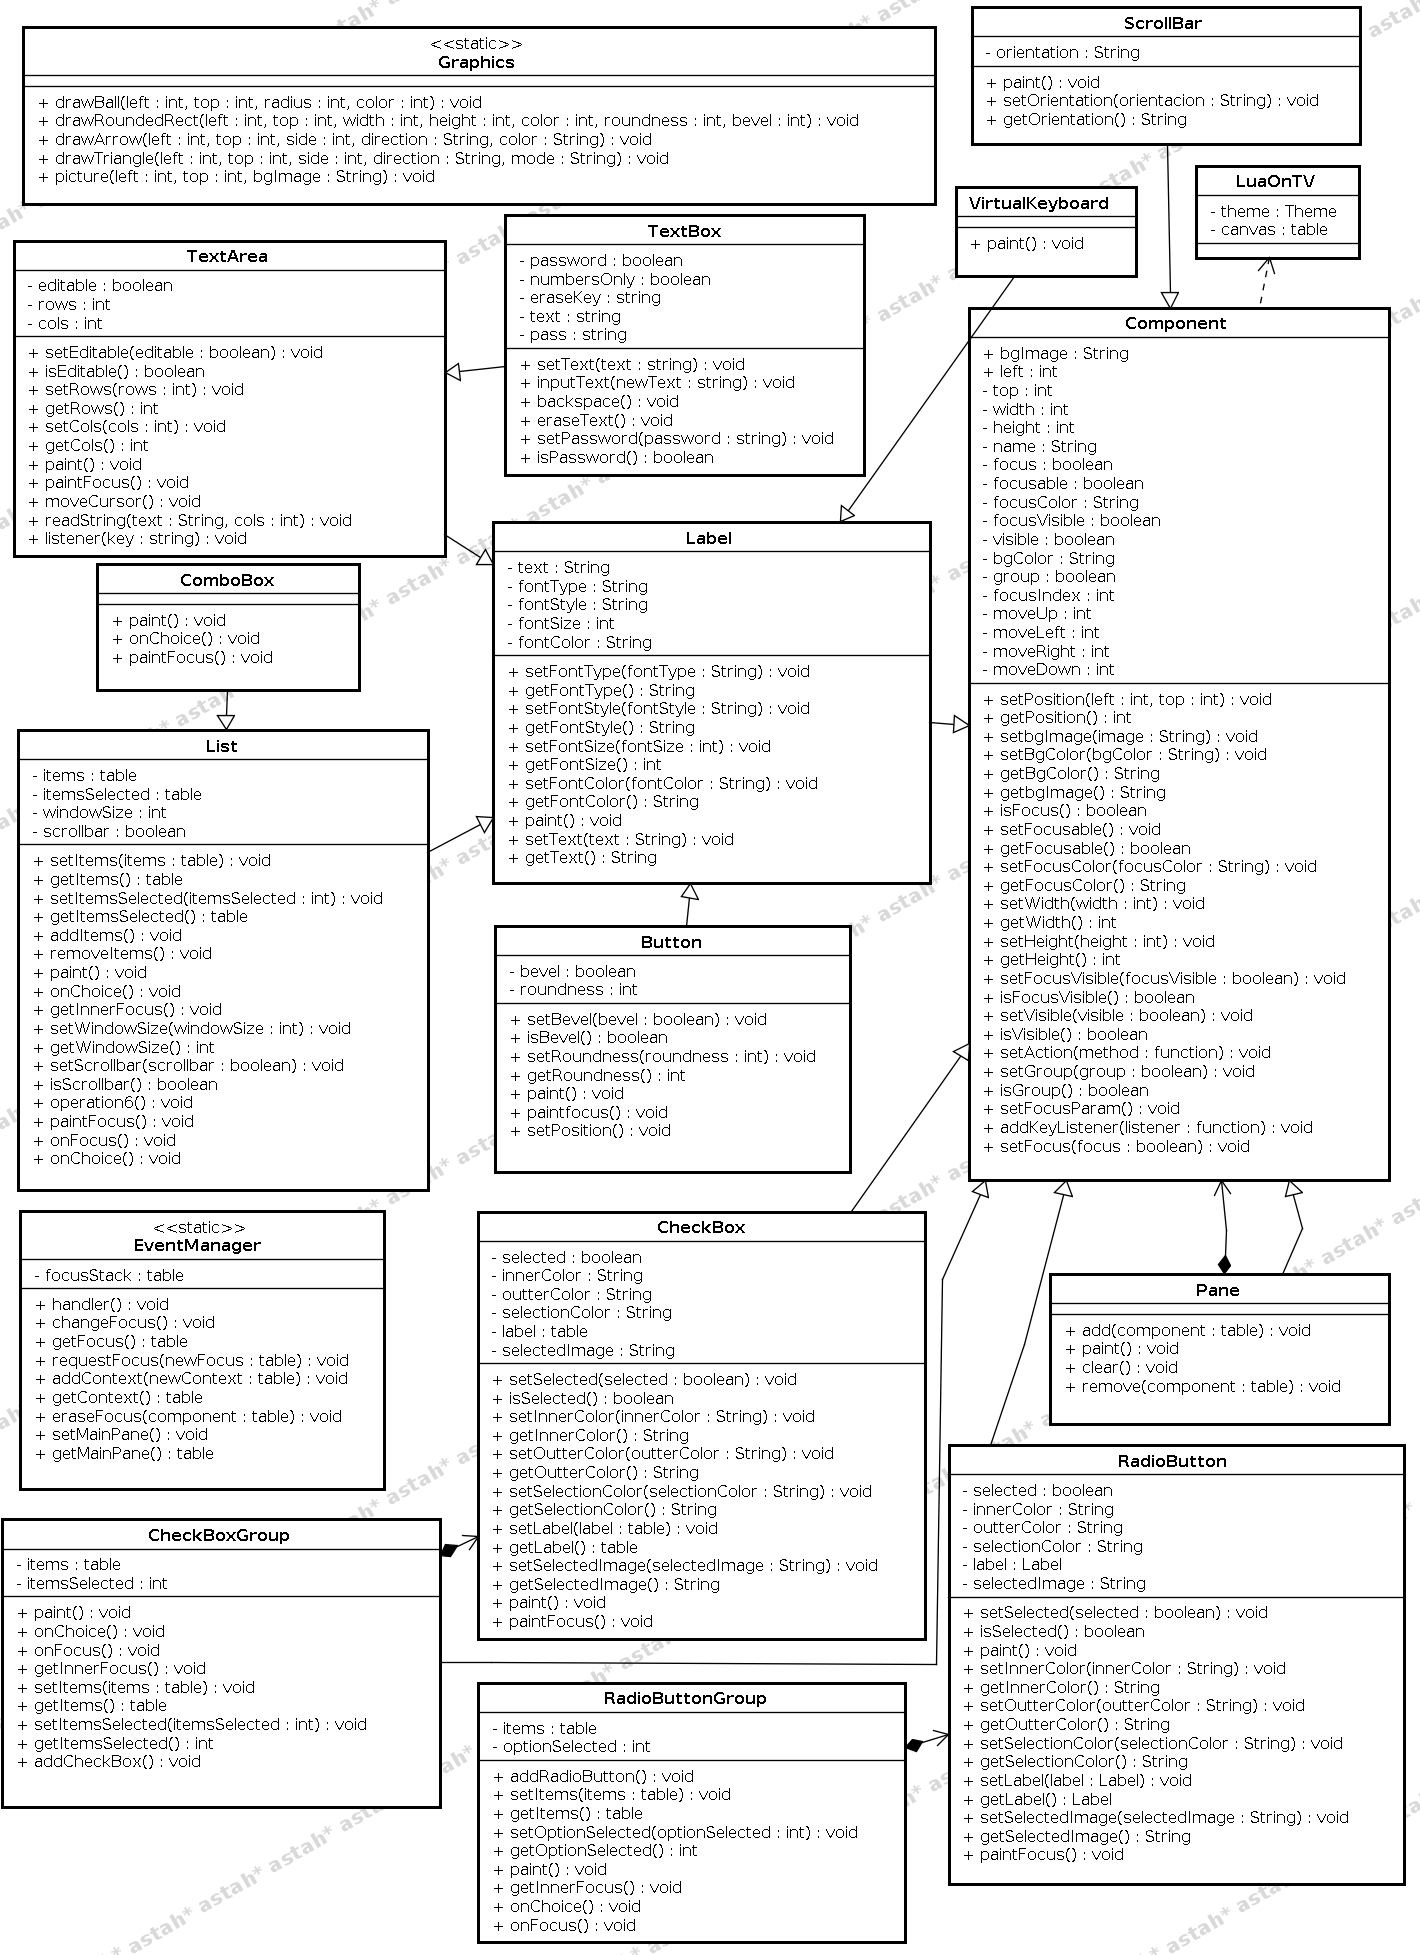
\includegraphics[width=1.12\textwidth]{LuaOnTV-Components.png}
	\captionof{figure}{Novo diagrama de classes do LuaOnTV}
	\label{fig:luaontv-classdiagram}
\end{center}

Neste diagrama, a classe \textit{EventManager} tem um papel fundamental no \textit{framework}, pois ela é responsável pelo tratamento
dos eventos ocorridos na aplicação, principalmente os eventos de pressionamento de teclas,
controlando a entrada de dados na tela e a navegação entre os campos por meio das teclas direcionais
do controle remoto. Desta forma, a Figura \ref{fig:event-manager-statemachine}
apresenta um gráfico de máquinas estados desta classe.

\begin{center}
	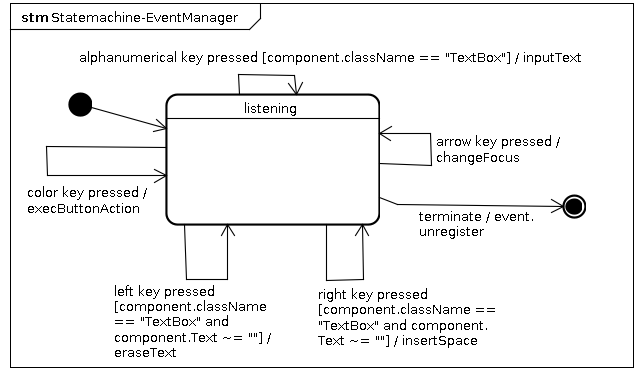
\includegraphics[width=0.8\textwidth]{LuaOnTV-Statemachine-EventManager.png}
	\captionof{figure}{Gráfico de Máquinas de Estados da classe \textit{EventManager}}
	\label{fig:event-manager-statemachine}
\end{center}

Um dos principais novos recursos implementados no LuaOnTV 
foi o suporte a temas. A Figura \ref{fig:luaontv-themes} apresenta as classes relacionadas a tal recurso.

\begin{center}
	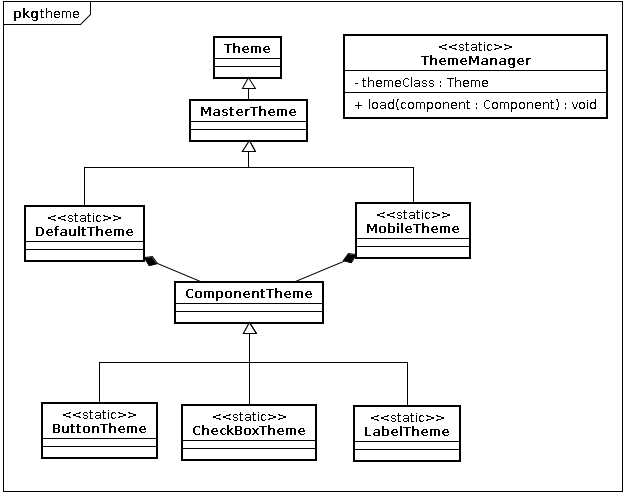
\includegraphics[width=0.8\textwidth]{LuaOnTV-Themes.png}
	\captionof{figure}{Classes relacionadas ao novo recurso de temas do LuaOnTV}
	\label{fig:luaontv-themes}
\end{center}

Como mencionado anteriormente, o LuaOnTV utiliza os módulos \textit{canvas} e \textit{event} do Ginga-NCL.
Assim, a Figura \ref{fig:luaontv-component-diagram} apresenta um diagrama de componentes,
mostrando como os elementos do LuaOnTV e do Ginga-NCL se relacionam.
O LuaOnTV possui dois pacotes principais: \textit{Components}, contendo as classes
que implementam os componentes visuais e não visuais; e \textit{Themes}, contendo
as classes que implementam os temas. O LuaOnTV cria uma camada
de abstração para os módulos \textit{canvas} e \textit{event} do Ginga-NCL, provendo
funcionalidades de mais alto nível.

\begin{center}
	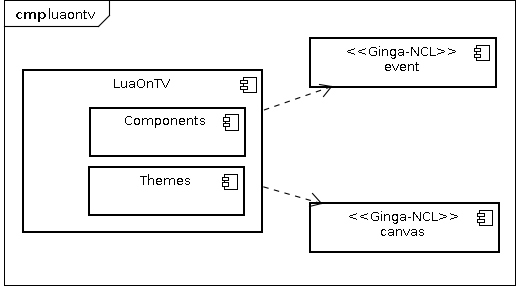
\includegraphics[width=0.7\textwidth]{LuaOnTV-Component-Diagram.png}
	\captionof{figure}{Diagrama de Componentes do LuaOnTV}
  \label{fig:luaontv-component-diagram}
\end{center}

